\begin{figure*}
\centering
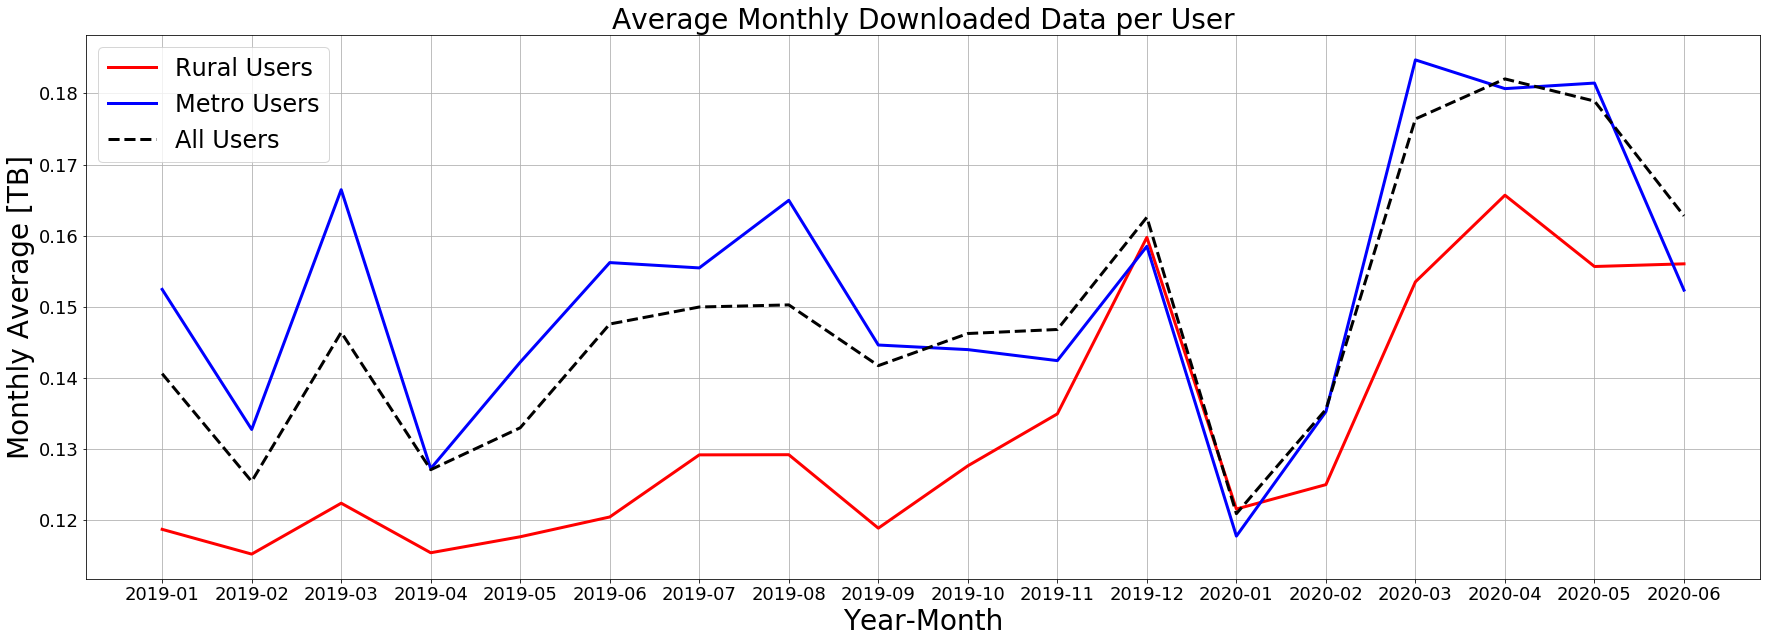
\includegraphics[width=1.0\linewidth]{figs/monthly_downloaded_data.png}
\caption{Graph showing the average consumption of downloaded data per user from 2019 to June 2020, partitioned by user county population.}
\label{fig:downloadmetro_rural}
\end{figure*}

\subsection{Analysis of Data Usage by Population Demographics}

\subsubsection{Average Monthly Usage}
A high-level overview of the effect of COVID-19 on internet usage can be seen by analyzing the average monthly downloaded data per user. As evidenced in Figure \ref{fig:downloadmetro_rural}, we notice a sizable increase in overall downloaded data in the months of March, April, and May. This increase is consistent across both county population levels, although it is more pronounced in metro areas: the 3 largest months by downloaded data occurred in the first 3 months of the pandemic. In rural areas, only one pandemic month is higher than December $2019$ levels.

Interestingly, in the fourth month of the pandemic, we notice a drop in overall downloaded data in metro areas, while rural areas remain constant. This drop coincides with the relaxation of many stay-at-home orders, indoor dining bans, and curfews in cities across the United States \cite{money2020la}, \cite{gov2020nyc}. 

\begin{figure*}
\centering
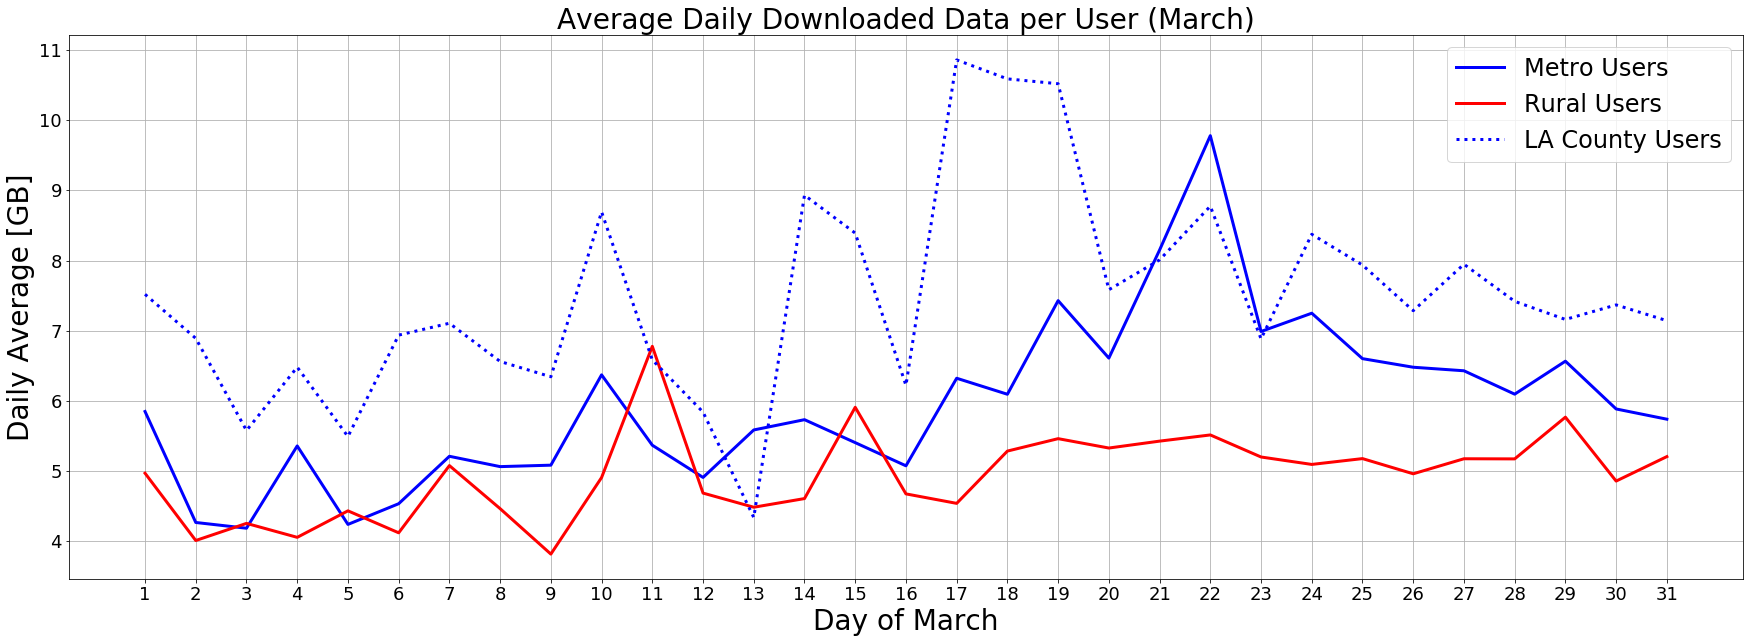
\includegraphics[width=1.0\linewidth]{figs/daily_downloaded_data.png}
\caption{Graph showing the daily consumption of downloaded data per user in March 2020 for those in metro and rural areas, as well as LA county.}
\label{fig:dailymetro_rural}
\end{figure*}

\subsubsection{Daily Data Usage}
While a month-by-month analysis allows us to observe larger trends over the course of the pandemic, focusing on average daily internet usage can allow to us to understand the public's reactions to various events. In particular, by analyzing daily averages over the course of the month of March, we can better understand the reactions to the various stay-at-home orders, school shutdowns, and curfews from an internet usage point-of-view. 

To this end, we present in Figure \ref{fig:dailymetro_rural} the daily average downloaded data usage for both metro and rural users. The first event we look to analyze is the White House first announcing its social distancing recommendations on March 16 for the entire country \cite{trump2020coronavirus}. Following this announcement, we observe that users in metro areas use a significantly larger amount of data than those in rural areas. In the first half of the month, there was no such difference (Figure \ref{fig:dailymetro_rural}). It is unsurprising that those in cities and other metro areas reacted to this recommendation more drastically than those in less populated areas. After all, cities such as New York City, San Francisco, and Los Angeles (LA) were among the hardest hit areas in the early weeks of the pandemic. 

For many of the aforementioned cities, various levels of lockdowns were put in place on top of the White House's recommendations. Therefore, we additionally investigate if we can correlate these local ordinances with county-level usage patterns. Los Angeles (LA) county has the most users in the MBA dataset ($n=44$), so we examine the daily average downloaded data per user for all those residing in LA (Figure \ref{fig:dailymetro_rural}). We observe the first large spike on March $14$, the day after many schools in the county shutdown \cite{haire2020LA}. March $14$ was a Saturday, so this spike is not due to remote learning. However, if schools were shut down by this date, then we can reasonably expect that various other aspects of society were shut down. For example, although the official order to ban indoor dining came later, by March $14$, many restaurants were were already closed \cite{eater2020}. This would suggest that the spikes we observe following government orders are due to people seeking entertainment from the internet over outside options.

We also notice a larger spike in the days following the national stay-at-home order. 


